\chapter{Four Lectures on Wave Mechanics}
\chapterprecis{Erwin Schr{\"o}dinger}

\makeoddhead{myheadings}{\emph{Schr{\"o}dinger}}{}{\thepage}
\makeevenhead{myheadings}{\thepage}{}{\emph{Four Lectures on Wave Mechanics}}

\renewcommand{\theequation}{\arabic{equation}}

\newenvironment{rcases}
  {\left.\begin{aligned}}
  {\end{aligned}\right\rbrace} % for eqn (14')

\section*{First Lecture\footnote{[London: Blackie \& Sons,
  Ltd. (1928) and New York: Chelsea (1982). Our excerpt includes only the first lecture.]}}

\subsection*{1. Derivation of the fundamental idea of wave mechanics from Hamilton's
analogy between ordinary mechanics and geometrical optics.}

\begin{figure}[h] % Figure 1
  \begin{center}
    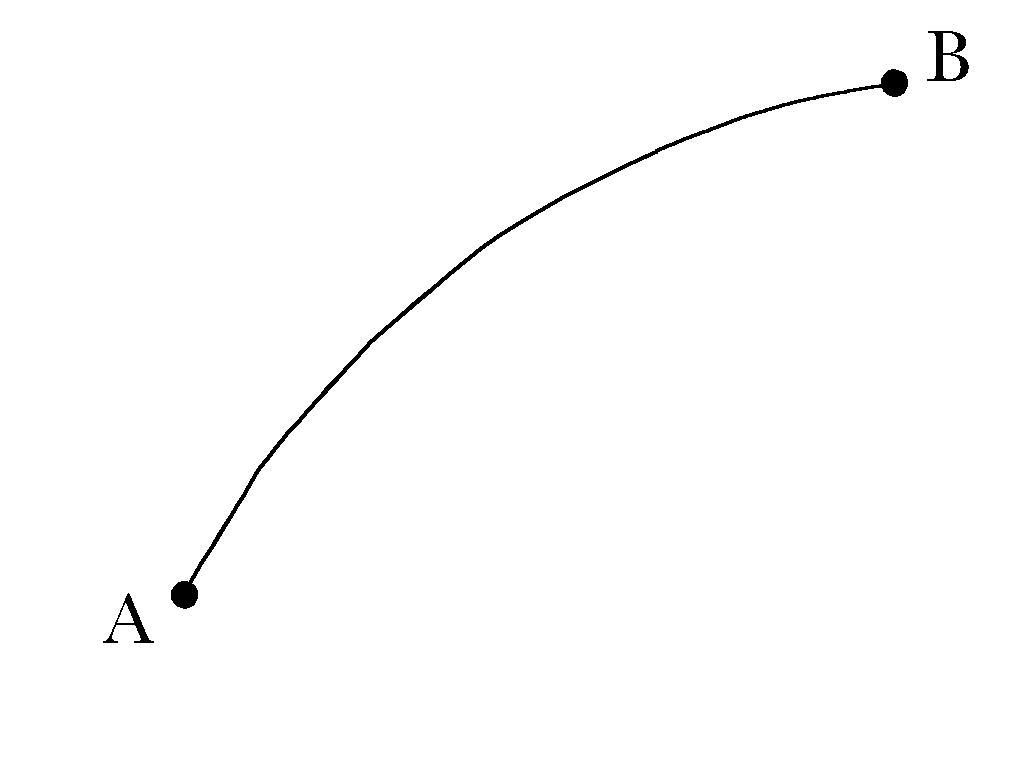
\includegraphics[width=1.98958in,height=1.47917in]{images/09_schroedinger/image035.png}
  \end{center}
  \caption*{\emph{FIGURE 1}}
\end{figure}

When a \emph{mass-point} $m$ moves in a conservative field of
force,
described by the potential energy
$V(x,y,z)$, then, if you let it
start from a given point $A$ with a given velocity, i.e.\ with a given
energy $E$, you will be able to get it into another arbitrarily
chosen point $B$ by suitably ``aiming,'' i.e.\ by letting it start in a
quite definitely chosen \emph{direction}. There is in general \emph{one}
definite dynamical orbit which leads from $A$ to $B$ \emph{with a
given energy}. This orbit possesses the property that
\begin{equation}
\delta \int_{A}^{B} \! 2T\,dt = 0 , % eqn (1)
\end{equation}
and is defined by this property (Hamilton's principle in the form given
to it by Maupertuis). Here $T$ means the kinetic energy of the mass-point,
and the equation means: consider the manifold of \emph{all} orbits
leading from $A$ to $B$ and subject to the law of conservation
of energy ($T + V = E$); among them the actual
dynamical orbit is distinguished by the fact that, \emph{for it} and for
all infinitely adjacent orbits of the manifold, the $\int_{A}^{B}$ has the \emph{same}
value[\ldots]. Calling $w= ds/dt$ the velocity of the mass-point, we have
\begin{equation*}
2T = mw^2 = m\left(\frac{ds}{dt}\right)^2 = 2(E-V) = \frac{ds}{dt}\sqrt{2m(E-V)}
\end{equation*}
by means of which equation (1) can be transformed into
\begin{equation} % eqn (2)
\delta \int_{A}^{B} \! \sqrt{2m(E-V)}\,ds = 0.\footnote{{[}This is equivalent to $\partial \int_{A}^{B} \! mw\,ds = 0$, since $2m(E-V)=2mT=m^2w^2$.}
\end{equation}
This form has the advantage that the variational principle is applied to
a purely geometrical integral, which does not contain the time-variable,
and further, that the condition of constant energy is automatically
taken care of.

\emph{Hamilton} found it useful to compare equation (2) with
\emph{Fermat's} principle, which tells us that in an optically
non-homogeneous medium the actual light rays, i.e.\ the tracks along
which energy is propagated, are determined by the ``law of minimum
time'' (as it is usually called).

Let fig.~1 \emph{now} refer to an optical medium of arbitrary
non-homogeneity, e.g.\ the earth's atmosphere; then, if you have a
searchlight at $A$, furnishing a well-defined beam, it will in
general be possible to illuminate an arbitrarily chosen point $B$
by suitably \emph{aiming} at it with the searchlight. There is one
definite light-path leading from $A$ to $B$, which obeys, and
is uniquely defined by, the law
\begin{equation}
\delta \int_{A}^{B} \! \frac{ds}{u} = 0.
\end{equation}
Here \emph{ds}, as before, means the element of the path, and $u$
is the velocity of light, a function of the co-ordinates $x, y, z$.

The two laws contained in equations (2) and (3) respectively become
\emph{identical}, if we postulate that
\begin{equation}
u = \frac{C}{\sqrt{2m(E-V)}} % eqn (4)
\end{equation}
where $C$ must be independent of $x, y, z$ but may
depend on $E$. Thus we have made a mental
picture of an optical medium, in which the manifold of possible
light-rays coincides with the manifold of dynamical orbits of a
mass-point $m$ moving \emph{with given energy} $E$ in a field of
force $V$(\emph{x},\emph{y},\emph{z}). The fact that \emph{u}, the
velocity of light, depends not only on the co\-or\-di\-nates but also on
$E$, the total energy of the mass-point, is of the utmost
importance.

This fact allows us to push the analogy a step farther by picturing the
dependence on $E$ as dispersion, i.e.\ as a dependence on
\emph{frequency}. For this purpose we
must attribute to our light-rays a definite frequency $\nu$,
depending on E. We will (arbitrarily) put
\begin{equation}
E = h\nu % eqn (5)
\end{equation}
($h$ being Planck's constant), without dwelling too much on this
assumption, which is very suggestive to modern physicists. Then this
non-homogeneous and dispersive medium provides in its \emph{rays} a
picture of \emph{all} the dynamical orbits of our particle. Now we can
proceed a stage farther, putting the question: can we make a small
``point-like'' \emph{light signal} move \emph{exactly} like our
mass-point? (Hitherto we have only secured the geometrical identity of
\emph{orbits}, quite neglecting the question of time-rate.) At first
sight this seems impossible, since the velocity of the mass point,
\begin{equation}
w = \frac{1}{m}\sqrt{2m(E-V)} , % eqn (6)
\end{equation}
is (along the path, i.e.\ with constant $E$) \emph{inversely}
proportional to the light-velocity $u$ (see equation (4); \emph{C}
depends on $E$ only). But we must remember that $u$ is of
course the ordinary \emph{phase}-velocity, whereas a small light-signal
moves with the so-called \emph{group-velocity}, say $g$, which is
given by
\begin{equation*}
\frac{1}{g}=\frac{d}{d\nu}\left(\frac{\nu}{u}\right) ,\footnote{[See section C of the de Broglie
chapter, particularly equation \ref{debsch}, p.~\pageref{debsch}.]}
\end{equation*}
or, in our case, following equation (5), by
\begin{equation}
\frac{1}{g} = \frac{d}{dE}\left(\frac{E}{u}\right). % eqn (7)
\end{equation}
\emph{We will try to make} $g=w$. The only means we have at our disposal
for this purpose is a suitable choice of $C$, the arbitrary
function of $E$ that appeared in equation (4). From (4), (6), and
(7), the postulate $g=w$ becomes
\begin{equation*}
\frac{d}{dE}\left(\frac{E\sqrt{2m(E-V)}}{C}\right) = \frac{m}{\sqrt{2m(E-V)}}
\equiv \frac{d}{dE}\left(\sqrt{2m(E-V)}\right) ;\footnote{{[}Schrödinger is really setting $1/g = 1/w$.
  The term on the left is $1/g$, while the middle term is
  $1/w$ (from eq. 6). But the middle term is also identically equal
  ($\equiv$) to the term on the right; thus the term on the left equals the
  term on the right. Moreover both terms are derivatives with respect to
  $E$. Since, then, the two quantities in parentheses have
  \emph{equal derivatives} with respect to $E$, \emph{they differ
  by at most a constant} (that is, by something that does not vary with
  $E$). The expression in the next line denotes that difference;
  therefore it ``is constant with respect to $E$.''{]}}
\end{equation*}
hence
\begin{equation*}
\left(\frac{E}{C}-1\right)\sqrt{2m(E-V)}
\end{equation*}
is constant with respect to $E$. Since $V$ contains the
co-or\-di\-nates and $C$ must be a function of $E$ only, this
relation can obviously be secured in a general way only by making the
first factor vanish. Hence
\begin{equation*}
\frac{E}{C}-1=0 \quad\quad \text{or} \quad\quad C = E ,
\end{equation*}
which gives equation (4) the special form
\begin{equation}\label{SchDeB}
u = \frac{E}{\sqrt{2m(E-V)}} . % eqn (8)
\end{equation}
This assumption about phase-velocity is the only one which will secure
absolute coincidence between the dynamical laws of motion of the
mass-point and the optical laws of motion of light-signals in our
imagined light-propagation. It is worthwhile mentioning that, according
to (8),
\begin{equation*}\tag{8'}
u = \frac{\text{energy}}{\text{momentum}}. % eqn (8')
\end{equation*}

\centerline{* * *}

Now the fundamental idea of wave-mechanics is the following. The
phenomenon, of which we believed we had given an adequate description in
the old mechanics by describing the motion of a mass-point, i.e.\ by
giving its co-ordinates $x, y, z,$ as functions of the
time variable $t$, is to be described correctly according to the
new ideas by describing a definite wave-motion, which takes place among
waves of the type considered, i.e.\ of the definite frequency and
velocity (and hence of the definite wave-length) which we ascribed to
what we called ``light'' in the preceding. The mathematical description
of a wave-motion will be furnished not by a limited number of functions
of the one variable $t$, but by a continuous manifold, so to speak,
of such functions, viz.\ by a function (or possibly several functions) of
$x, y, z,$ and $t$. These functions will be
subject to a \emph{partial} differential equation, viz.\ to some sort of
\emph{wave equation}.

\centerline{* * *}

\subsection{2. Ordinary mechanics only an approximation, which no longer holds for
very small systems.}

In replacing the ordinary mechanical description by a wave-mechanical
description our object is to obtain a theory which comprises both
ordinary mechanical phenomena, in which quantum conditions play no
appreciable part, and, on the other hand, typical quantum phenomena. The
hope of reaching this object resides in the following analogy.
Hamilton's wave-picture, worked out in the way discussed above, contains
\emph{something} that corresponds to ordinary mechanics, viz.\ the
\emph{rays} correspond to the mechanical \emph{paths}, and
\emph{signals} move like \emph{mass-points}. But the description of a
wave-motion in terms of \emph{rays} is merely an approximation (called
``geometrical optics'' in the case of light-waves). It only holds if the
structure of the wave phenomenon that we happen to be dealing with is
coarse compared with the wave-length, and as long as we are only
interested in its ``coarse structure.'' The detailed fine structure of a
wave phenomenon can never be revealed by a treatment in terms of rays
(``geometrical optics''), and there always exist wave-phenomena which
are altogether so minute that the ray-method is of no use and furnishes
no information whatever. Hence in replacing ordinary mechanics by wave
mechanics we may hope on the one hand to retain ordinary mechanics as an
approximation which is valid for the coarse ``macro-mechanical''
phenomena, and on the other hand to get an explanation of those minute
``micro-mechanical'' phenomena (motion of the electrons in the atom),
about which ordinary mechanics was quite unable to give any information[\ldots].

The step which leads from ordinary mechanics to wave mechanics is an
advance similar in kind to Huygens' theory of light, which replaced
Newton's theory. We might form the symbolic proportion:
\begin{center}
\begin{align*}
\text{Ordinary mechanics} &: \text{Wave mechanics =}\\
\text{Geometrical optics} &: \text{Undulatory optics.}\\
\end{align*}
\end{center}
Typical quantum phenomena are analogous to typical wave phenomena like
diffraction and interference.

For the conception of this analogy it is of considerable importance that
the failure of ordinary mechanics does occur in dealing with very
\emph{tiny} systems. We can immediately control {[}i.e., ascertain{]}
the order of magnitude at which a complete failure is to be expected,
and we shall find that it is exactly the right one. The wave-length, say
$\lambda$, of our waves is (see equations (5) and (8))
\begin{equation}
\lambda = \frac{u}{\nu} = \frac{h}{\sqrt{2m(E-V)}} = \frac{h}{mw} ,
\end{equation}
i.e.\ Planck's constant divided by the momentum of the
mass-point.\footnote{{[}See Section A of the de Broglie chapter.{]}} Now take, for
the sake of simplicity, a circular orbit of the hydrogen-model, of
radius $a$, but not necessarily a ``quantized'' one. Then we have
by ordinary mechanics (without applying quantum rules):
\begin{equation*}
mwa = n\frac{h}{2\pi} , 
\end{equation*}
where $n$ is any real positive number (which for Bohr's quantized
circles would be 1, 2, 3 \ldots ; the occurrence of $h$ in the
latter equation is for the moment only a convenient way of expressing
the order of magnitude). Combining the last two equations, we get
\begin{equation*}
\frac{\lambda}{a} = \frac{2\pi}{n}.
\end{equation*}
Now in order that we may be justified in the application of ordinary
mechanics it is necessary that the dimensions of the path calculated in
this way should turn out to be large compared with the wave-length. This
is seen to be the case as long as the ``quantum number'' $n$ is
large compared with unity. As $n$ becomes smaller and smaller, the
ratio of $\lambda$ to $a$ becomes less and less favourable. A
complete failure of ordinary mechanics is to be expected precisely in
the region where we actually meet with it, viz.\ where $n$ is of the
order of unity, as it would be for orbits of the normal size of an atom
($10^{-8}$ cm).

\subsection{3. Bohr's stationary energy-levels derived as the frequencies of proper
vibrations of the waves.}

Let us now consider the wave‑mechanical treatment of a case which is
inaccessible to ordinary mechanics; say, to fix our ideas, the
wave‑mechanical treatment of what in ordinary mechanics is called the
motion of the electron in the hydrogen atom.

In what way are we to attack this problem?

Well, in very much the same way as we would attack the problem of
finding the possible movements (vibrations) of an elastic body. Only, in
the latter case the problem is complicated by the existence of two types
of waves, longitudinal and transverse. To avoid this complication, let
us consider an elastic fluid contained in a given enclosure. For the
pressure, $p$, say, we should have a wave equation
\begin{equation}
\nabla^2p - \frac{1}{u^2}\ddot{p} = 0 , %eqn (10)
\end{equation}
\emph{u} being the \emph{constant} velocity of propagation of
longi­tudinal waves, the only waves possible in the case of a fluid. We
should have to try to find the most general solution of this partial
differential equation that satisfies certain boundary
conditions at the surface of the vessel. The
standard way of solving is to try
\begin{equation*}
p(x,y,z,t) = \psi(x,y,z)e^{2\pi i\nu t} ,
\end{equation*}
which gives for $\psi$ the equation
%
\begin{equation*}\tag{10'}
\nabla^2\psi + \frac{4\pi^2\nu^2}{u^2}\psi = 0
\end{equation*}
%
$\psi$ being subject to the same boundary conditions as $p$. We
then meet with the well- known fact that a regular solution $\psi$
satisfying the equation and the boundary conditions cannot be obtained
for \emph{all} values of the co­efficient of $\psi$, i.e.\ for
\emph{all} frequencies $\nu$, but only for an infinite set of
discrete frequencies \emph{$\nu$\textsubscript{1}, $\nu$\textsubscript{2},
$\nu$\textsubscript{3}, \ldots , $\nu$\textsubscript{k}, \ldots ,} which are
called the characteristic or proper
frequencies (\emph{Eigenfrequenzen}) of the problem or of the body.
Call $\psi_k$ the solution (ordinarily unique apart
from a multiplying constant) that belongs to $\nu_k$,
then---since the equation and the boundary conditions are homogeneous---
%
\begin{equation}
p = \sum_{k}c_k \psi_k e^{2\pi i(\nu_kt+\theta_k)} % eqn (11)
\end{equation}
%
will, with arbitrary constants $c_k$, $\theta_k$, be a more general solution and indeed be
\emph{the} general solution, if the set of quantities
($\psi_k, \nu_k$) is complete [\ldots].

In the case of the waves which are to replace in our thought the motion
of the electron, there must also be some quantity $p$, subject to a wave 
equation like equation (10),
though we cannot yet tell the physical meaning of $p$. Let us put
this question aside for the moment. In equation (10) we shall have to
put
\begin{equation*}\tag{8}
u = \frac{E}{\sqrt{2m(E-V)}} .\footnote{{[}Compare Section C of the de Broglie chapter, especially equation 4.{]}}
\end{equation*}
This is not a constant; it depends (1) on $E$, that is,
essen­tially on the frequency $\nu$ ($= E/h$); (2) on the coordinates
$x, y, z,$ which are contained in the potential energy
$V$. These are the two complications as compared with the simple
case of a vibrating fluid body considered above. Neither of them is
serious. By the first, the dependence on $E$, we are restricted in
that we can apply the wave equation only to a function $p$ whose
dependence on the time is given by
\begin{equation*}
p \sim e^{\frac{2\pi iEt}{h}}
\end{equation*}
whence
\begin{equation}
\ddot{p} = - \frac{4\pi^2E^2}{h^2}p .
\end{equation}
We need not mind that, since it is precisely the same assumption
(\emph{Ansatz}) as would be made in any case in the standard method of
solution. Substituting from (12) and (8) in (10) and replacing the
letter $p$ by $\psi$ (to remind us that now, just as before, we
are investigating a function of the coordinates only), we obtain
\begin{equation}
\nabla^2\psi + \frac{8\pi^2m}{h^2}(E-V)\psi = 0 . % eqn (13)
\end{equation}
We now see that the \emph{second} complication (the depen­dence of
$u$ on $V$, i.e.\ on the co‑or\-di\-nates) merely results in a
somewhat more interesting form of equation (13) as compared with (10'),
the quantity multiplying $\psi$ being no longer a \emph{constant,} but
depending on the coordinates. This was really to be expected, since an
equation that is to embody the mechanical problem cannot very well help
containing the potential energy of the problem. A simplification in the
problem of the ``mechanical'' waves (as compared with the fluid problem)
consists in the absence of boundary conditions. 

I thought the latter
simplification fatal when I first attacked these questions. Being
insufficiently versed in mathematics, I could not imagine how proper
vibration frequencies could appear \emph{without} boundary conditions.
Later on I recognized that the more complicated form of the coefficients
(i.e.\ the appearance of $V(x,y,z)$) takes charge, so to speak, of
what is ordinarily brought about by bound\-a\-ry con\-di\-tions, name\-ly, the
selection of definite values of $E$.

I cannot enter into this rather lengthy mathematical discussion here,
nor into the detailed process of finding the solutions, though the
method is practically the same as in ordinary vibration problems,
namely: introducing an appropriate set of coordinates (e.g.\ spherical or
elliptical, according to the form of the function $V$) and putting
$\psi$ equal to a \emph{product} of functions, each of which contains
one coordinate only. I will state the result straightforwardly for the
case of the hydrogen atom. Here we have to put
\begin{equation}
V = -\frac{e^2}{r} + \text{const.,}  % eqn (14)
\end{equation}
$r$ being the distance from the nucleus. Then it is found that not
for all, but only for the following values of $E$, is it possible
to find regular, one‑valued, and finite solutions:
\begin{equation*}\tag{14'}
\begin{rcases}
  \text{(A) } E_n &= \text{const.} - \frac{2\pi^2me^4}{h^2n^2}; n=1,2,3,4... \\
  \text{(B) } E &> \text{const.} % eqn (14')
\end{rcases}
\end{equation*}
The constant is the same as in (14) and is (in non‑rela­tivistic wave
mechanics) meaningless, except that we cannot very well give it the
value which is usually adopted for the sake of simplicity, \emph{viz}.
zero. For then all the values (A) would become negative. And a negative
frequency, if it means anything at all, means the same as the positive
frequency of the same absolute value. Then it would be mysterious why
all positive frequencies should be allowed, but only a discrete set of
negative ones. But the question of this constant is of no importance
here.

You see that our differential equation automatically selects as the
allowed $E$‑values (A) the energy‑levels of the elliptic orbits
quantized according to Bohr's theory; (B) all energy‑levels belonging to
hyperbolic orbits. This is very remarkable. It shows that, whatever the
waves may mean physically, the theory furnishes a method of quantization
which is absolutely free from arbitrary postulates that this or that
quantity must be an integer.

\centerline{* * *}


\section*{Remarks}


In 1928, Erwin Schrödinger was invited to address the Royal Institution in London, where he presented a series of lectures introducing his notion of “wave mechanics.” As befitting such an introduction, his emphasis is on the broad outlines of the theory rather than detailed accounts of application. That said, by the end of the first lecture, which is all that is presented here, he has already stated what he takes to be one of the key signs of the novelty and success of his approach. Schrödinger announces this novelty in the title of a series papers published two years earlier, “Quantization as an eigenvalue [or ‘proper value’] problem.”\footnote{``Quantisierung als Eigenwertproblem,'' 
\emph{Ann. Phys.\ }\textbf{79}, 361; \textbf{79}, 489; \textbf{80}, 437; \textbf{81}, 109 (1926).}

Quantization, of course, is a name for the fact we have been dealing with since learning about Bohr’s model of the atom, namely, the restriction of electrons to discrete orbits with definite energies, what Bohr called “stationary states.” De Broglie’s notion of some kind of wave associated with the particle suggests that the motion of a particle may be explained in terms of the refraction of this wave. The forces acting on a particle would thus be due to differences in something analogous to the refractive index of transparent materials, and the discreteness of its allowed orbits would result from the fact that the wave must be in phase with itself in its course about the nucleus; it must be a standing wave. Schrödinger carries this analogy even farther, with his mathematical formulation of a differential equation completely describing the motion of the electron, a wave equation.

The equation, he points out in section 3, cannot be “solved” for just any values of its parameters, but, in the case of the term for the wave’s frequency, only for “an infinite set of discrete frequencies […] called the characteristic or proper frequencies (\emph{Eigenfrequenzen}) of the problem.” (The energies associated with these frequencies would then be the "proper values" or "eigenvalues" of the problem.) This set of frequencies can be likened to the harmonic series for a vibrating string, though, as we will see, there are other more spatially complicated forms of periodicity in the atom.

Those complications aside, most of what Schrödinger is saying is clear, even if it still requires a good deal of interpretation. Some of his argument, however, relies on mathematical relations and techniques that may be unfamiliar. In section 1, Schrödinger makes use of the calculus of variations and some reasoning from de Broglie to derive an expression for the phase-velocity of the electron. In section 3, he uses a variety of techniques for solving his differential equation including separation of variables and a complex exponential. Accounts of these relations and techniques follow.

\subsection*{Calculus of Variations (Sec. 1): Least Action and Least Time}

Leibniz in the \emph{Essay on Dynamics} had defined ``moving action''
(\emph{l'action motrice}) as the joint product of the ``formal effect''
in a motion---mass times a distance moved, or $ms$---and the
velocity of the movement, $v$ or $s/t$. (Note that
  action is only defined for a whole motion, covering a finite distance
  in a finite time.) Thus the quantity of action $Q$ associated
with any motion at constant speed can be expressed as $msv$ or,
equivalently, as
\begin{equation*}
Q = msv = ms\cdot\frac{s}{t}=m\frac{s}{t}\cdot\frac{s}{t}\cdot t = mv^2\cdot t.
\end{equation*}
Since kinetic energy, $T$, is $\frac{1}{2}mv^2$, we
can also express the action associated with such a motion as
\begin{equation*}
Q = 2T\cdot t.
\end{equation*}
If the speed is not constant, we must \emph{integrate} the above
expression over time, and thus the action $Q$ will be
\begin{equation*}
Q = \int_{A}^{B} 2T\,dt,
\end{equation*}
where $A$ and $B$ refer respectively to the times at the beginning and the
end of the motion.

\emph{The Principle of Least Action}\footnote{It may have been
  discovered by Leibniz himself, but the direct evidence for that is
  lost. It was first published by Pierre-Louis Maupertuis in 1744.}
(which Schrödinger cites as ``Hamilton's principle'') states as a 
fundamental dynamical law that the particulars of any motion
are always arranged so as to \emph{minimize} the total action associated
with that motion. This is a very powerful principle. Together with the
Principle of Conservation of Total Mechanical Energy it can be shown to
produce, \emph{as a consequence}, Newton's Laws of Motion and hence the
rest of mechanics. So in beginning his treatment with these
principles, Schrödinger is going back to an alternative
conceptualization for the very foundations of mechanics.

To see what it means for action to be minimized, consider a freely moving body 
which traverses a path between A and B. Now consider the \emph{difference} $\Delta Q$ between the
action calculated over that actual path and over some other path (with
different velocities and kinetic energies $T'$) between the same
two endpoints:
\begin{equation*}
\Delta Q = \int_{A}^{B}\!2T'\,dt-\int_{A}^{B}\! 2T\,dt = \Delta\int_{A}^{B}\!2T\,dt.
\footnote{In this equation $A$ and $B$ are shorthand for the
  times at which the body is at the $A$ and $B$ of the figure.
  They are not specified as the same for the two paths; only the points
  themselves are.}
\end{equation*}
Next, let the hypothetical path be only \emph{infinitesimally} removed
from the actual path. Then the difference in action will likewise become
infinitesimal. It is represented by the special notation
\begin{equation*}
\delta Q = \partial \int_{A}^{B} \! 2T\,dt.
\end{equation*}
For the symbol $\delta$ read ``the \emph{variation of}.''

The variational principle states that for the \emph{actual} path, and
only for that path, the variation $\delta Q$ will equal
\emph{zero}. Symbolically, this condition is stated
\begin{equation*}
\delta Q\int_{A}^{B} \! 2T\,dt = 0.
\end{equation*}
It appears as equation (1) in Schrödinger's lecture.

As we indicated above, this is analogous to using calculus to find a
maximum or minimum point for a function of one variable $y=f(x)$, for 
here a strict analogue to the variational principle
also holds. That is, for any maximum or minimum point in such a
function, one could say that
\begin{equation*}
\delta y = 0.
\end{equation*}
For, recall that at any maximum or minimum point the first derivative of
the function, $dy/dx$, must equal \emph{zero}. But a very small
change $\Delta y$ in a function caused by a very small change $\Delta x$
is closely approximated by $\Delta y = (dy/dx)\Delta x$. As a result, at a 
maximum or minimum point
\emph{the variation of the function is, to a first
approximation, equal to zero}.
Thus one might expect that, analogously, the variation of the action
integral was zero for the actual, least-action, path. Mathematicians
managed to prove that this was indeed so.

The \emph{Principle of Least} \emph{Time} applies to light, and
states that the path actually taken by a light beam in passing from A to
B is always a path of minimum overall time, compared to neighboring
paths joining the same endpoints. It too can be restated in the
``variational'' form:
\begin{equation*}
\delta \int_{A}^{B} \! dt = 0.
\end{equation*}

Note that if the light velocity is $u = s/t$, then
$t = s/u$ and $dt = ds/u$; so that the principle may also be expressed:
\begin{equation*}
\delta \int_{A}^{B} \! \frac{ds}{u} = 0.
\end{equation*}
This appears as equation (3) in Schrödinger's lecture.

A related reformulation turns the time-integral of equation (1) into
an integral over space, equation (2): note that $msv = (mv)s$, so that action can
also be thought of as \emph{momentum times distance traveled}. If
$v$ is not constant, but is given as a function of the distance
traveled, we can integrate, getting
\begin{equation*}
Q = \int_{A}^{B} \! mv\,ds ,
\end{equation*}
where $A$ and $B$ correspond to the starting-point and endpoint of the motion,
such that for that path the integral over distance \emph{s} will always
be equal to the time-integral over $T$,
\begin{equation*}
Q = \int_{A}^{B} \! 2T\,dt ,
\end{equation*}
from above. Thus the variations of both of these integrals will equal
zero for the same, least-action path.

Schrödinger uses this spatial identity of the paths and some reasoning
borrowed from de Broglie about group and phase velocity to derive equation
(8), which will prove essential for later reasoning. In fact, here, there
is a strict likeness to something familiar. In the final section of his
``Remarks on the preceding papers by Mr. Bernoulli'' (\emph{Mechanics,} 207-230),
Euler confesses he does not know how to solve the wave equation for a string
that varies in thickness along its length, i.e., when the velocity term is itself 
a function of the spatial term: ``the determination of the movement of these strings appears to be
beyond our powers'' (230). This is precisely what we will have in Schrödinger's
wave equation (10), where the velocity $u$ defined in equation (8) contains 
the potential $V$, which varies with position, in particular, with distance from
the center of the atom.

\subsection*{Solving Differential Equations (Sec. 3): Separation of Variables and Complex Exponentials}

\emph{A. Notation.} As was just noted above, in one sense, Schrödinger's first approach to the wave 
equation, in equation (10), could not be more traditional. It, too, relates the 
spatial derivative to the temporal by a simple multiplicative factor, as we can
see with a simple rearrangement:
\begin{equation*}\tag{10'}
\nabla^2p = \frac{1}{u^2}\ddot{p}.
\end{equation*}
Two pieces of notation may be unfamiliar. The first is the double-dot notation ($\ddot{p}$), which
stands for the second derivative of the function with respect to time. The second, $\nabla$, is 
simply a shorthand for the sum of the individual spatial derivatives. In three-dimensional space, 
then, $\nabla^2p$ just means
\begin{equation*}
\frac{\partial^2p}{\partial x^2} + \frac{\partial^2p}{\partial y^2} + \frac{\partial^2p}{\partial z^2}.
\end{equation*}
In the one-dimensional case of the vibrating string and its transverse wave, we 
could think of this second spatial derivative geometrically as the curvature: the more
intense the curvature, the more intensely was that portion of the string subject to
the restoring force. In the two-dimensional case of a stretched drumhead, we can imagine
it being struck in the center and the disturbance thus produced spreading radially in all directions
in the plane. Here, too, the wave is transverse: the drumhead moves up and down, but the
wave moves from the center to the periphery. Since the wave moves across the surface of the 
drumhead, the relevant ``curvature'' in this case must
be measured with respect to two dimensions, say $x$ and $y$. The portions of the wave (call it 
$\psi$) 
moving directly along the $y$-direction alone (say, away from and toward the drummer)
would have a non-zero value for $\frac{\partial^2\psi}{\partial y^2}$
and a zero value for $\frac{\partial^2\psi}{\partial x^2}$, and conversely for the portions of
the wave moving along the $x$-direction alone (left to right); but the portion of the wave moving along a line
from the center pointing forward \emph{and} to the right would have non-zero degrees 
of curvature expressed 
in the second partials for both $x$ and $y$. Finally, in three dimensions, it is possibly
easier to think of a longitudinal wave, such as a pressure wave, where the wave
function's value at any point in space represents the pressure of the medium at that point.
Here, clearly, the wave equation will have to measure something analogous to the string's 
or the drumhead's curvature in all \emph{three} spatial dimensions at once in order to
correctly account for the propagation of that wave in time.

So much for notation. As noted above, Schrödinger employs the technique of separation of variables
to solve his equation and also uses a complex exponential. We will describe both before considering
how they are applied in this case.

\vspace{5pt}
\emph{B. Separation of Variables.} The idea is that in order to solve a partial differential
equation, one begins by trying out a function that is the product
of two other functions of only some of the variables, for instance, of space and time. 
The usefulness of this can be seen from the product rule $(fg)' = fg' + f'g$. If $f$ and
$g$ are functions of space and time respectively, then their derivatives with respect to
the other coordinates are zero and that latter term drops out---e.g., $\frac{\partial}{\partial x}(f(x)g(t)) =
f \cdot 0 + f'(x)g(t) = f'(x)g(t)$---leaving equations that are easier to solve.


As for what, beyond a desire for an easier solution, might induce us to think the 
function we are looking for could be expressed as a product, we can note that this is
just the form we see in the standing-wave solutions to the one-dimensional wave equation for
the vibrating string. For a string free to move up and down along the $y$-axis and stretched along the $x$-axis from 0 to 2$\pi$, the second harmonic could have the form $y = sin(x)cos(\pi t).$ The following pictures 
show how this function appears at times $t = 0, 1, 2$.
\begin{figure}[h]
  \centering
  \subfloat{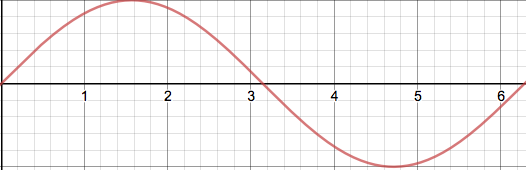
\includegraphics[width=1.75333in]{images/09_schroedinger/harmonic0.png}}
   \hspace{.2in}
  \subfloat{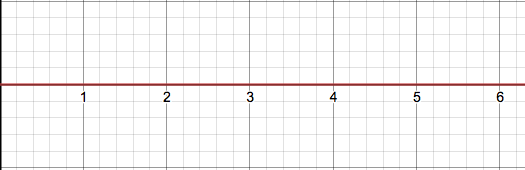
\includegraphics[width=1.75in]{images/09_schroedinger/harmonic1.png}}
   \hspace{.2in}
  \subfloat{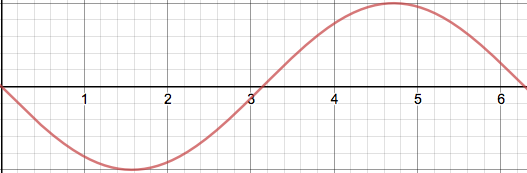
\includegraphics[width=1.75667in]{images/09_schroedinger/harmonic2.png}}
\end{figure}
The sinusoidal shape stays fixed in place, even as its amplitude diminishes to 0 and then passes 
over into the negative. But this is just what the separated form of the wave-function says: there 
is a shape, a function of the spatial coordinate, that does not vary with time, and a changing amplitude-factor that is the same throughout the whole spatial extent of the wave-function.

In the case of Schrödinger's wave equation (10), he considers a ``trial'' solution that is the product
of distinct spatial and temporal parts. We've already noted how this might facilitate finding a solution.
A futher simplification comes from the way the function of time is expressed, as a \emph{complex exponential}.

\vspace{5pt}
\emph{C. Complex Exponentials.} You will likely have encountered Euler's number, $e$, the base of the natural logarithm. And you may have encountered the imaginary unit $i = +\sqrt{-1}$, used in the definition of the \emph{complex numbers}, which have the form $a + bi$, where $a$ and $b$ are real numbers. Euler proved that, if it has any meaning at all, the expression $e^{i\theta}$ should be interpreted as equal to the complex number $\cos{\theta} + i\sin{\theta}$. If we imagine the complex numbers as represented in a plane, then the complex exponentials lie on the unit circle about the origin, and $\theta$ represents the arc length proceeding counter-clockwise around the circumference, starting from the point $1 + 0i$. 

Given the simplicity of the rules for differentiating and integrating the exponential, and the ease
with which it could be recast as a simple real-valued sinusoidal function (i.e.,
by ignoring the imaginary part), the complex exponential earned itself a place in the physicist's
mathematical toolbox. For our purposes, it is almost sufficient simply to know the rule
\begin{equation*}
de^{ix} = d(\cos{x} + i\sin{x}) = -\sin{x}\, dx + i\cos{x}\, dx = ie^{ix}\, dx.
\end{equation*}
Given this, it's easy to see that the factor $-4\pi^2\nu^2$ in (10') comes from differentiating the product
$\psi(x,y,z)e^{2\pi i\nu t}$ twice with respect to time, as does the similar factor in (12), after
the substitution of $E/h$ for the frequency $\nu$. Late in the next chapter, we will consider
more about how the complex form of the solution affects interpretation.

\vspace{5pt}
\emph{D. The Form of the Solutions.} In equation (11), Schrödinger points out what would be the
general solution if this were
simply the problem of finding the pressure waves in ``an elastic fluid in a given enclosure.''
There are a lot of terms, but if one imagines sinusoidal functions for each of the $\psi_k$, each
with its own amplitude $c_k$, and ignores the time-function and its frequencies and phase angles, 
it looks a lot like Bernoulli's 
formulation for the shape of the vibrating string. Bernoulli's component waves, of course, have
wavelengths that are submultiples of the length of the string, and in this way, his ``solution''
to the problem already includes the so-called ``boundary conditions,'' as does Schrödinger's
equation (11) in a general way (in its selection of frequencies $\nu_k$).

But by the time he gets to equation (14'), Schrödinger is referring to a far more definite set
of solutions. Along the way, he notes two ``complications'' and one ``simplification'' of the
wave equation for the electron in comparison with the fluid problem. One we noted above, the
dependency of the ``velocity'' term $u$ on the spatial coordinates, and the likeness between
this and the problem Euler imagined, of the string of varying thickness. But it's the simplification
that poses what could have been a ``fatal'' problem. In the case of Bernoulli's solution we just
mentioned (as well as in that of Euler's reformulation), the boundary conditions did some of the
work of selecting from among the infinite scope of possible solutions. Here, the electron could
be \emph{anywhere in space,} like one of de Broglie's ``pilot waves.''

In this first lecture to the Royal Institution introducing the very idea of wave mechanics to
a scientifically literate, but not necessarily expert, audience, Schrödinger is understandably
less than completely informative concerning ``the detailed process of finding the solutions,'' 
which would entail a ``rather lengthy mathematical discussion.'' Nonetheless, given the significant
work we have done both this year and last to understand wave phenomena and mechanics, we should
pause to fill in a little bit of the story here.

In somewhat naive terms, beginning from de Broglie, we might have imagined the wave threading
around the nucleus of the atom in one orbital plane, its crests and troughs aligning with one 
another. The functions that are unique solutions to Schrödinger's wave equation at a given energy level,
however, are rather more geometrically complicated. Schrödinger is a bit more forthcoming about
their form in the second lecture:

\begin{quote}
The detailed behavior of the ``elliptic'' functions within the said region [i.e., those belonging
to bound electrons, near the nucleus] cannot very well be described in a unique way, for the
following reason. To \emph{one} value of $E_n$ there belongs in general not only one, but 
precisely $n^2$ independent solutions of the wave equation. From the mathematical point of
view this is an exception due to the particular form of the potential energy $V$, especially to
its spherical symmetry[\ldots]. Since the equation is linear and homogeneous, any linear aggregate
with quite arbitrary coefficients [cf. equation (11)] will also be a solution belonging to the
\emph{same} proper value[\ldots]. To give an example: from a set of solutions whose node-surfaces
[i.e., surfaces with the same magnitude] are (1) concentric spheres, (2) co-axial cones, (3)
planes passing through the cone-axis, you can form other solutions, in which the concentric
spheres and co-axial cones are replaced by two sets of confocal paraboloids. This is only one
of the simplest cases. In general, taking arbitrary coefficients, the system of node-surfaces
will be \emph{much} more complicated.
\end{quote}

Two notes here: 1) the ``magnitude'' mentioned in the interpolation is the modulus squared
of the complex number that is the value of the wave-function: if the number is $a + bi,$
this is the non-negative real number $a^2 + b^2$; 2) the wave-function is in general spread
out in space, such that the node-surfaces formed by choosing a particular magnitude of the
function give only some of the information about the geometry of the function, as a
weather map might indicate gross features of the atmospheric pressure in a large region 
by tracing several lines of constant pressure (isobars). Perhaps you will have seen
representations of the higher-order ``orbitals'' in a book of chemistry. It is these 
shapes and details about the atomic behavior of electrons that Schrödinger's equations
allowed physicists to understand, even as the difficult work of interpreting the
physical meaning of the wave equation for a material particle was just beginning.
 
